% !TeX spellcheck = en_GB
\documentclass{beamer}\mode<presentation>{\usetheme{AMSBolognaFC}}
\setbeamertemplate{bibliography item}{\insertbiblabel}

\usepackage{common}

\newcommand{\labN}{5}
\newcommand{\labGroup}{https://gitlab.com/pika-lab/courses/ds/ay2122}
\newcommand{\labRepo}{\labGroup/lab-\labN}

\title[L\labN{} -- Presentation]{L\labN{} -- Presentation}
%
\subtitle[SD]{Distributed Systems / Technologies}
%
\author[Ciatto \and Omicini]
{\emph{Giovanni Ciatto} \and Andrea Omicini\\
\texttt{giovanni.ciatto@unibo.it \and andrea.omicini@unibo.it}}
%
\institute[DISI, Univ. Bologna]
{Dipartimento di Informatica -- Scienza e Ingegneria (DISI)\\\textsc{Alma Mater Studiorum} -- Universit{\`a} di Bologna a Cesena}
%
\date[A.Y. 2021/2022]{Academic Year 2021/2022}

\setbeamercovered{transparent}

\AtBeginSection[]
{
\begin{frame}[c]\frametitle{Next in Line\ldots}
%    \begin{multicols}{2}
        \tableofcontents[sectionstyle=show/shaded, subsectionstyle=show/hide, subsubsectionstyle=hide/hide]
%    \end{multicols}
\end{frame}
}

\AtBeginSubsection[]
{
    \begin{frame}[c]\frametitle{Next in Line\ldots}
        %    \begin{multicols}{2}
        \tableofcontents[sectionstyle=show/shaded, subsectionstyle=show/hide, subsubsectionstyle=show/hide]
        %    \end{multicols}
    \end{frame}
}

\begin{document}

\maketitle

\begin{frame}[c]\frametitle{Outline}
    % \begin{multicols}{2}
	    \tableofcontents[sectionstyle=show/show, subsectionstyle=show/show, subsubsectionstyle=show/show]
    % \end{multicols}
\end{frame}

%\section{Motivation}
%
%\begin{frame}[allowframebreaks]
%\frametitle{Motivation}
%
%    \begin{itemize}
%        \item Some motivation here
%
%    \end{itemize}
%
%\end{frame}

\section{Remote Procedure Call}

\begin{frame}[allowframebreaks]
    \frametitle{RPC -- Remote Procedure Call}

    \begin{block}{Intuitive definition}
        \begin{itemize}
            \item A client synchronously invokes a remote function on a server
            %
            \begin{itemize}
                \item and waits for its completion
            \end{itemize}

            \item Invocations may carry arguments, completions may carry results

            \item A server is supposed to be waiting for remote invocations

            \item Request--response metaphor
        \end{itemize}
    \end{block}

    \centering

    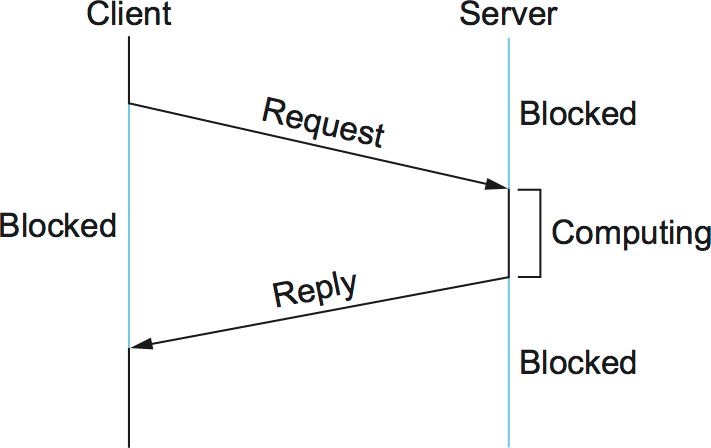
\includegraphics[width=.8\linewidth]{img/rpc.png}

    \framebreak

    \begin{alertblock}{Important aspects}
        \begin{enumerate}
            \item Arguments and results must be exchanged over the network
            %
            \begin{itemize}
                \item Passage by reference is impossible:
                %
                \begin{itemize}
                    \item the client and the server do not share the same addressing space
                \end{itemize}

                \item Passage by value is the only option
                %
                \begin{itemize}
                    \item copies must be transferred over the network
                \end{itemize}
            \end{itemize}

            \item The client and the server are temporally coupled
            %
            \begin{itemize}
                \item the server must be available to serve the client
            \end{itemize}

            \item From the perspective of the clients' caller
            %
            \begin{itemize}
                \item the client and the server have the same interface
                \item the client acts as a proxy for the server
            \end{itemize}
        \end{enumerate}
    \end{alertblock}

\end{frame}

\begin{frame}[allowframebreaks]
    \frametitle{RPC -- Marshalling and Unmarshalling}

    \centering

    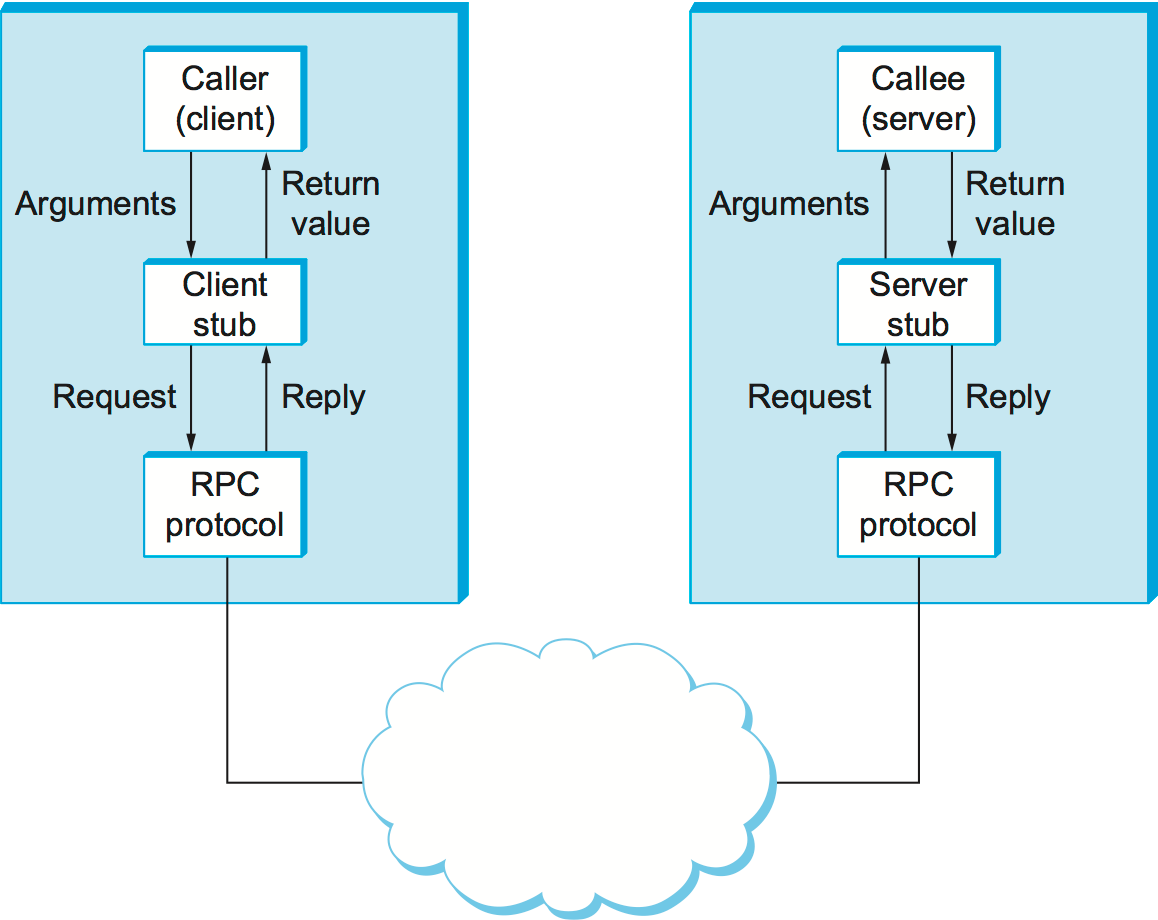
\includegraphics[width=.7\linewidth]{img/rpc-2.png}

    \framebreak

    \begin{block}{To support RPC we need}
        \begin{description}
            \item[a client stub] --- marshalling the arguments, unmarshalling the results, and blocking/resuming the client

            \item[a server stub] --- unmarshalling the arguments, marshalling the results, and resuming/blocking the server

            \item[a transport protocol] --- to transfer arguments and results over the network
        \end{description}
    \end{block}

    \framebreak

    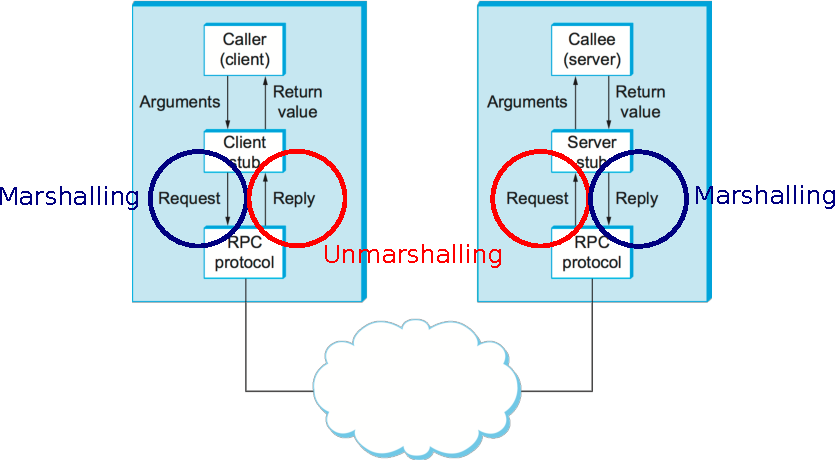
\includegraphics[width=\linewidth]{img/rpc-3.pdf}

    \begin{block}{Marshalling and unmarshalling, informal definition}
        \begin{description}
            \item[marshalling] --- serialization of data to be sent over the network

            \item[unmarshalling] --- deserialization of data received from the network
        \end{description}
    \end{block}

\end{frame}

\section{(De)Serialization}

\begin{frame}[allowframebreaks]
    \frametitle{About (De)Serialisation}

    \begin{block}{Informal definition}
        \begin{description}
            \item[Serialization] --- converting in-memory objects into char/byte sequences
            \item[Deserialization] --- converting chars/bytes back into in-memory objects of some \emph{type}
        \end{description}
    \end{block}

    \bigskip

    \begin{alertblock}{Interoperability among different platform}
        Attained via common \emph{data representation format}
        %
        \begin{itemize}
            \item[eg] textual formats such as XML, JSON, YAML
            \item[eg] binary formats such as BSON, XDR, AVRO's, Protobuf's
        \end{itemize}
    \end{alertblock}

\end{frame}

\begin{frame}[allowframebreaks]
\frametitle{(D)Encoding vs. (De)Serialising}

    \begin{block}{Data representation format $\neq$ Encoding}
        \begin{description}
            \item[(D)Econders] just provide a particular means to interpret bytes/chars
            \item[(De)Serialisers] also provide some means to represent \emph{data structures}
        \end{description}
        %
        \begin{itemize}
            \item[!] All data-representation formats explicitly or implicitly rely on some encoding
            %
            \begin{itemize}
                \item[eg] most textual data representation formats rely on \texttt{UTF-8} or \texttt{UTF-16}
            \end{itemize}
        \end{itemize}
    \end{block}

\end{frame}

\begin{frame}[allowframebreaks]
    \frametitle{Working with Charsets and Encodings in Java}
    \begin{block}{Charset vs. Encoding}
        \begin{description}
            \item[Charset] dictates how bytes are interpreted as chars within strings
            \item[Encoding] rules how to represent byte/char strings using some charset
        \end{description}
    \end{block}

    \begin{examples}{Most notable charsets}
        \begin{itemize}
            \item ASCII \url{https://www.asciitable.it/}
            \item UTF-8 \url{https://www.utf8-chartable.de/}
            \item \alert{UTF-16} \url{https://asecuritysite.com/coding/asc2}
            %
            \begin{itemize}
                \item[!] modern programming languages use UTF-16 for strings
            \end{itemize}
        \end{itemize}
    \end{examples}

    \begin{examples}{Most notable encodings}
        \begin{itemize}
            \item identity (i.e. each character represents itself)
            \item identity + some escape sequences (e.g. \texttt{$\backslash{}$n}, \texttt{$\backslash{}$t}, etc.)
            \item URL/Percent encoding
            \item base64 encoding (\url{https://en.wikipedia.org/wiki/Base64})
            \item \ldots
        \end{itemize}
    \end{examples}

    \begin{block}{Standard Charsets in Java}
        Two notable charset-related classes:
        %
        \begin{description}
            \item[\href{https://docs.oracle.com/en/java/javase/17/docs/api/java.base/java/nio/charset/Charset.html}{\texttt{java.nio.charset.\textit{Charset}}}] | represent a charset
            \item[\href{https://docs.oracle.com/en/java/javase/17/docs/api/java.base/java/nio/charset/StandardCharsets.html}{\texttt{java.nio.charset.\textit{StandardCharsets}}}] | contains a number of standard instances of \texttt{Charset}
        \end{description}
    \end{block}

    \begin{block}{URL (Percent) Encoding and Decoding in Java}
        Two notable URL-econding-related classes in Java:
        %
        \begin{description}
            \item[\href{https://docs.oracle.com/en/java/javase/17/docs/api/java.base/java/net/URLEncoder.html}{\texttt{java.net.\textit{URLEncoder}}}] | aimed at encoding strings in percent encoding
            \item[\href{https://docs.oracle.com/en/java/javase/17/docs/api/java.base/java/net/URLDecoder.html}{\texttt{java.net.\textit{URLDecoder}}}] | aimed at decoding percent-encoded strings
        \end{description}

        \medskip

        How to use them:
        %
        \begin{description}
            \item[\texttt{URLEncoder.encode(string, charset)}] | converts \texttt{string} in a URL-encoded string using \texttt{charset}
            \item[\texttt{URLDecoder.decode(string, charset)}] | parses \texttt{string} as a URL-encoded string using \texttt{charset}
        \end{description}
    \end{block}

    \framebreak

    Usage example:
    %
    \lstinputlisting[language=Java,morekeywords={var}]{./code/UrlEncodeExample.java}
\end{frame}

\begin{frame}%[allowframebreaks]
    \frametitle{About (De)Serialisation in Java}

    \begin{itemize}
        \item Java SE is quite well suited for (de)serialisation
        %
        \begin{itemize}
            \item[eg] Java's custom data serialization facilities (a.k.a. \texttt{DataInputStream} \& \texttt{DataOutputStream})
            \item[eg] Java's binary serialization framework (a.k.a. \texttt{ObjectInputStream} \& \texttt{ObjectOutputStream})
            \item[eg] Java's \texttt{javax.xml.*} package
        \end{itemize}

        \vfill

        \item However, the JVM ecosystem is plenty of open-source libraries for JSON / YAML support

    \end{itemize}

    \vfill

    \begin{block}{JVM technologies for (de)serialisation}
        \href{https://github.com/google/gson}{\emph{Gson}},
        \href{https://github.com/FasterXML/jackson}{Jackson},
        \href{https://avro.apache.org/docs/1.10.0/}{Apache Avro},
        \href{https://developers.google.com/protocol-buffers}{Google's Protocol Buffers},
        \href{https://thrift.apache.org/}{Thrift}
    \end{block}
    %
    \begin{itemize}\small
        \item[!] Avro, Thrift, and ProtoBuff are actually full-fledged tools for Middleware development
    \end{itemize}

\end{frame}

\begin{frame}[allowframebreaks]
    \frametitle{General (De)Serialisation Library}

    You can expect a (de)serialisation library to expose these functionalities:
    %
    \bigskip
    %
    \begin{itemize}
        \item \emph{convert} objects of some \emph{type} into strings, according to some format

        \bigskip

        \item \emph{write} objects of some \emph{type} onto output streams, according to some format

        \bigskip

        \item \emph{parse} strings in some format into objects of some type \emph{type}

        \bigskip

        \item \emph{read} input streams, parse them according to some format, outputting objects of some \emph{type}
    \end{itemize}

    \framebreak

    \begin{block}{(De)Serialisation usually involves the construction of an AST}
        \hint{AST = abstract syntax tree}
        \begin{description}
            \item[Serialisation:] in-memory object $\rightarrow$ AST $\rightarrow$ byte/char string
            \item[Deserialisation:] byte/char string $\rightarrow$ AST $\rightarrow$ in-memory object
        \end{description}
        %
        \medskip
        %
        \begin{itemize}
            \item Libraries usually include some \emph{types} to let developers build the AST
            %
            \begin{itemize}
                \item[eg] \texttt{JsonElement} and its subclasses in Gson
                \item[eg] \texttt{JsonNode} and its subclasses in Jackson
            \end{itemize}

            \smallskip

            \item Most libraries are able to read/write several \emph{concrete} syntaxes for the same AST
            \begin{itemize}
                \item[eg] Jackson may read/write XML, JSON, or YAML from a \texttt{JsonNode}
            \end{itemize}

            \smallskip

            \item[!] When the concrete syntax is XML, the AST is a.k.a. \emph{Domain Object Model} (DOM)
        \end{itemize}
    \end{block}
\end{frame}

\begin{frame}%[allowframebreaks]
    \frametitle{(De)Serialisation in Strongly-Typed Languages}

    \begin{itemize}
        \item Serialisation and deserialisation are somewhat \emph{asymmetrical} in OOP libraries

        \vfill

        \item While serialising, libriaries know both:
        %
        \begin{itemize}
            \item the actual type of the in-memory object to be serialised
            \item the target data representation format
        \end{itemize}

        \vfill

        \item While deserialising, libraries only know:
        %
        \begin{itemize}
            \item the actual data representation format of the to-be-parsed string
            \item while the target type the wanna-be in-memory object is unknown
        \end{itemize}

        \vfill

        \item[$\rightarrow$] Developers must always specify the \emph{expected type} upon deserialisation
        %
        \begin{itemize}
            \item subtle technicality with deep implications
        \end{itemize}
    \end{itemize}

\end{frame}

\begin{frame}[allowframebreaks]
    \frametitle{Gson API}

    \begin{block}{Main classes}
        \begin{description}
            \item[\href{https://www.javadoc.io/doc/com.google.code.gson/gson/latest/com.google.gson/com/google/gson/JsonElement.html}{\texttt{com.google.gson.\textit{JsonElement}}}] | root type for data AST
            \item[\href{https://www.javadoc.io/doc/com.google.code.gson/gson/latest/com.google.gson/com/google/gson/Gson.html}{\texttt{com.google.gson.\textit{Gson}}}] | entry point for (de)serialising \texttt{JsonElement}s
            \item[\href{https://www.javadoc.io/doc/com.google.code.gson/gson/latest/com.google.gson/com/google/gson/GsonBuilder.html}{\texttt{com.google.gson.\textit{GsonBuilder}}}] | a builder for configuring \texttt{Gson} objects
        \end{description}
    \end{block}

    \begin{exampleblock}{\texttt{JsonElement} type hierarchy}
        \centering
        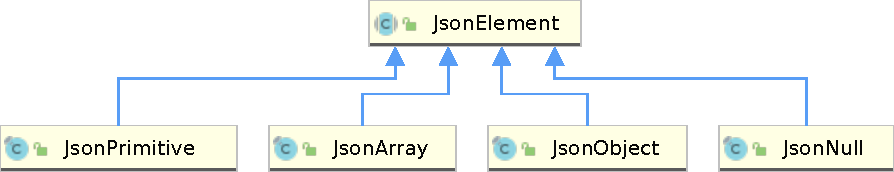
\includegraphics[width=.5\linewidth]{./img/JsonElementCompact.pdf}
    \end{exampleblock}

    \begin{block}{\texttt{Gson} relevant methods}
        \begin{description}
            \item[\texttt{new Gson()}] | creates a new instance of \texttt{Gson}
            \item[\texttt{gson.toJson(object)}] | generates a JSON string from an AST (or object)
            \item[\texttt{gson.fromJson(string, Type.class)}] | parses an AST (or an instance of \texttt{Type}) out of a JSON string
            \item[\texttt{gson.toJson(object, writer)}] | converts an AST (or object) into a JSON string and writes it into the provided writer
            \item[\texttt{gson.fromJson(reader, Type.class)}] | reads an AST (or an instance of \texttt{Type}) from the provided reader
        \end{description}
    \end{block}

    \begin{exampleblock}{\texttt{JsonElement} relevant methods}
        \centering
        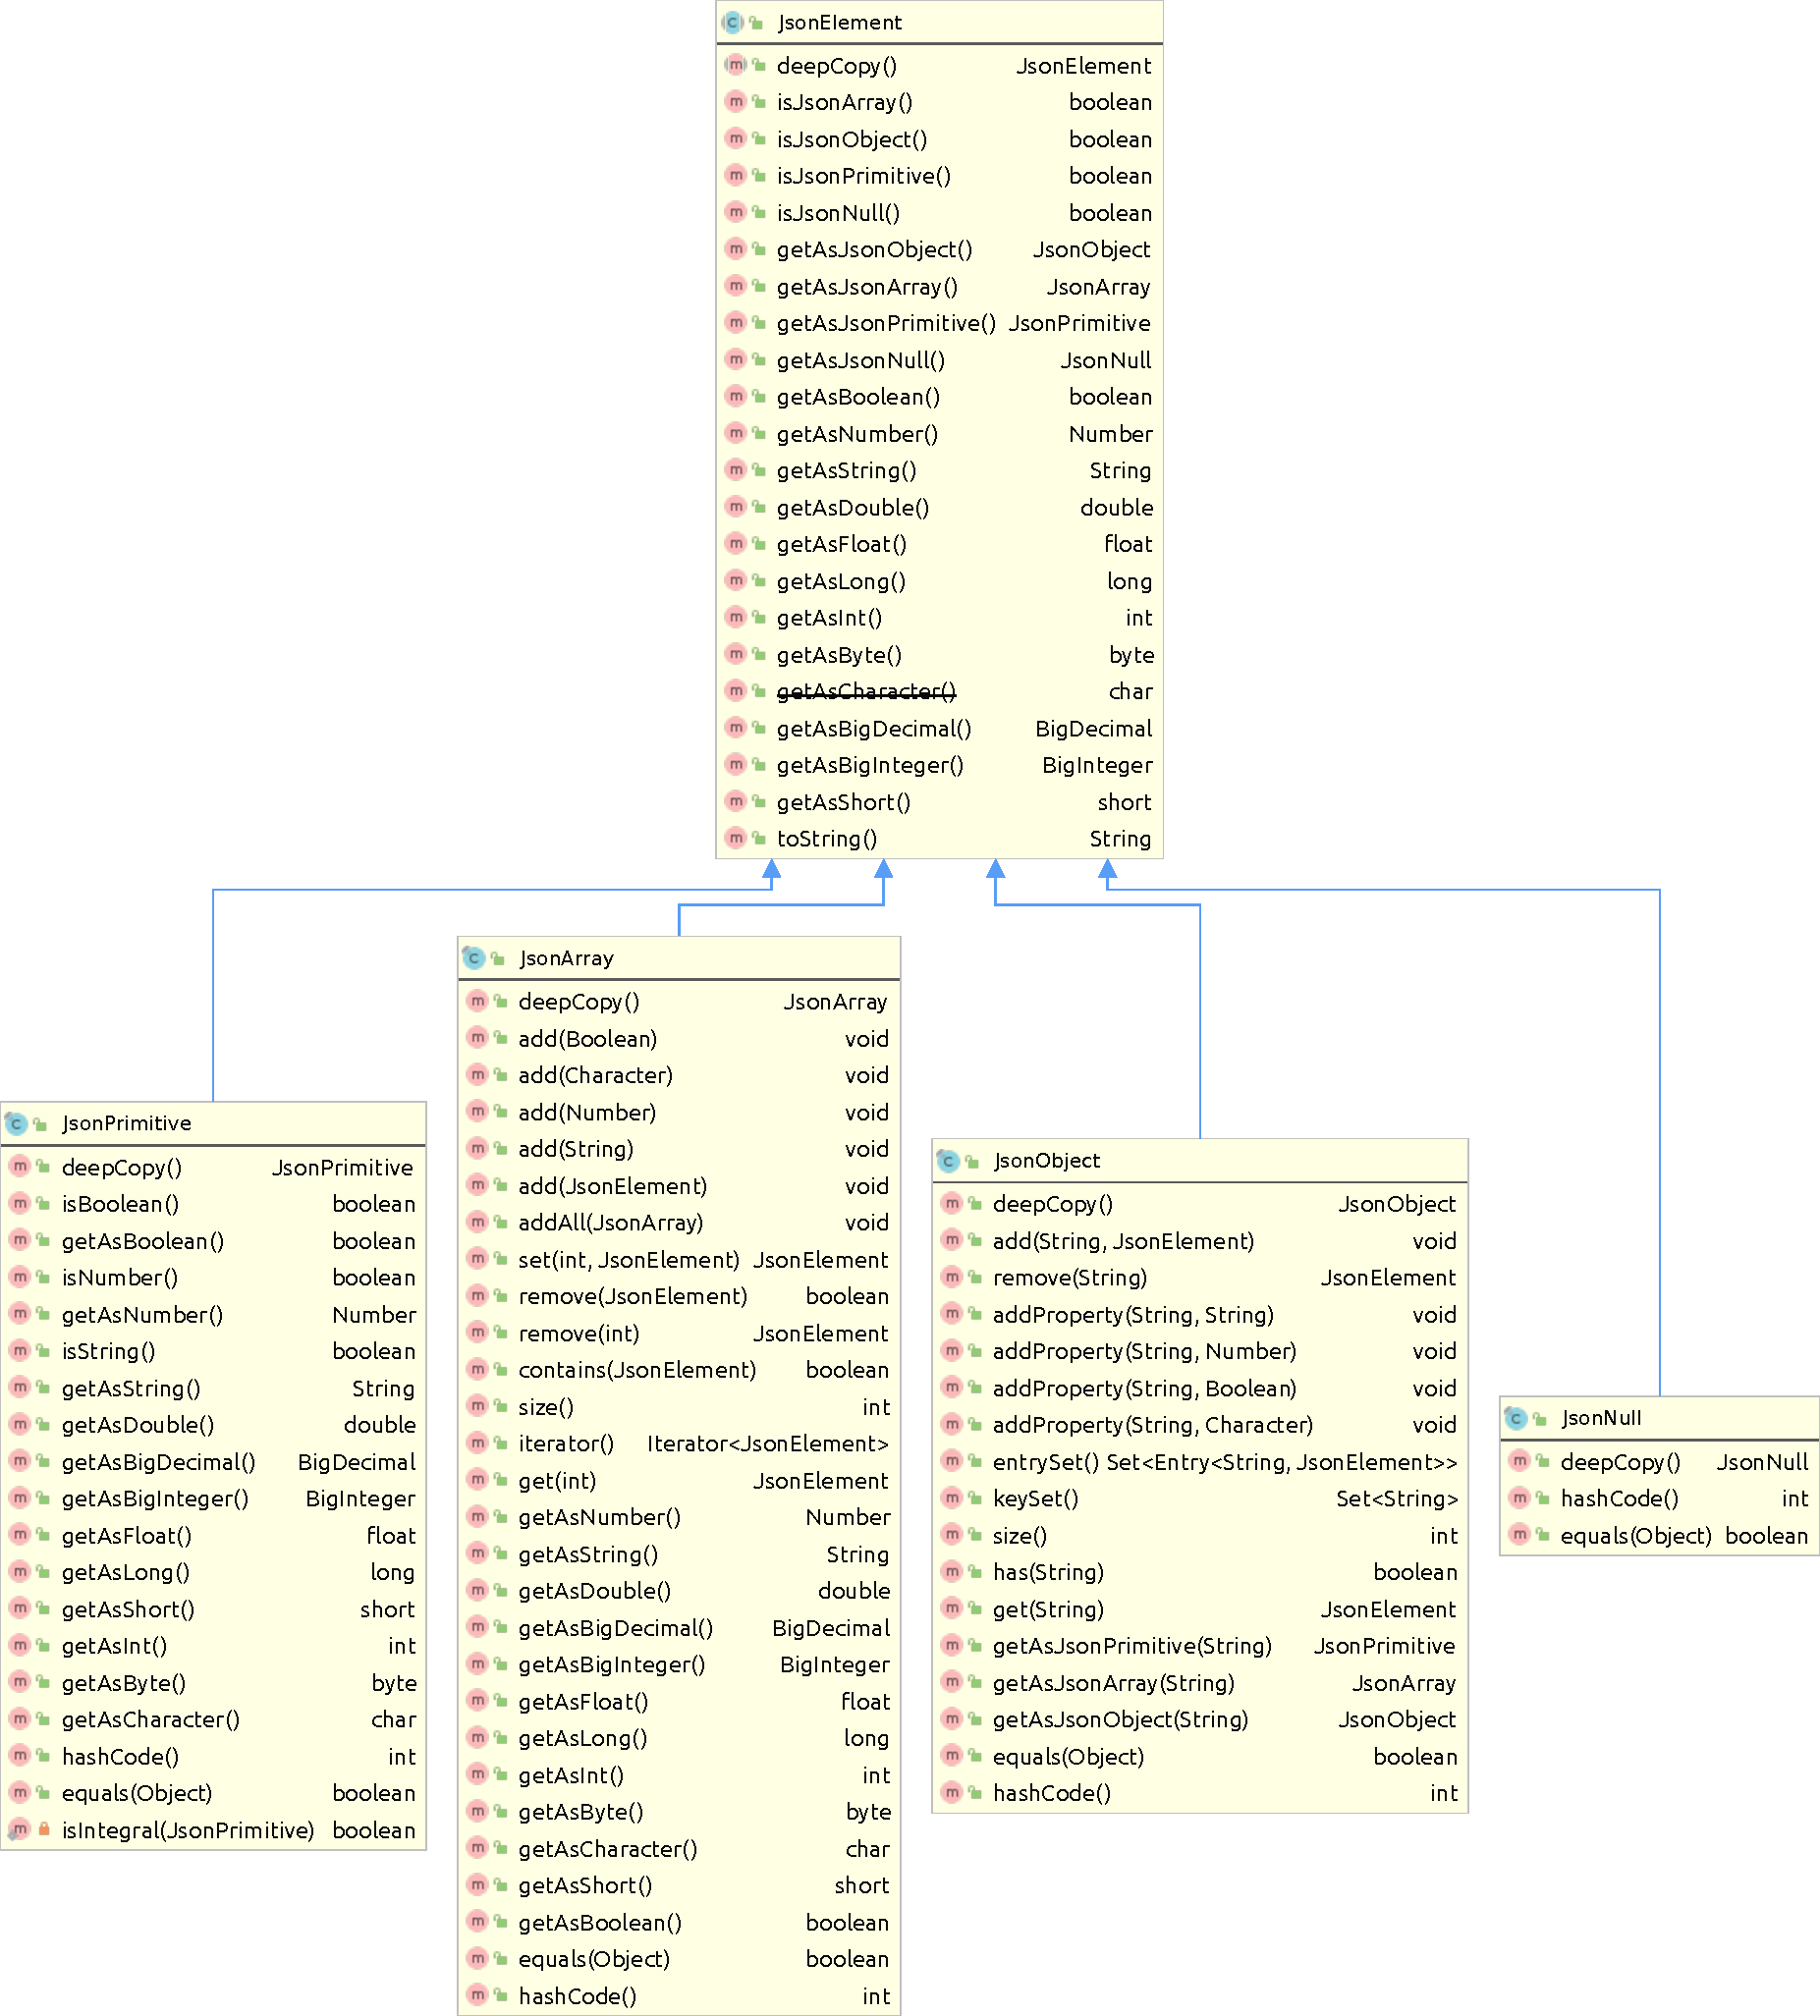
\includegraphics[height=.7\textheight]{./img/JsonElement.pdf}
    \end{exampleblock}

\end{frame}

\begin{frame}[allowframebreaks]
    \frametitle{Gson Example}

    Consider a simple data structure such as:
    %
    \lstinputlisting[language=Java,morekeywords={var}]{./code/Person.java}

    \framebreak

    A serialiser for \texttt{Person}s can be designed as follows:
    %
    \lstinputlisting[language=Java,morekeywords={var},basicstyle=\tiny\ttfamily]{./code/PersonSerializer.java}

    \framebreak

    A deserialiser for \texttt{Person}s can be designed as follows:
    %
    \lstinputlisting[language=Java,morekeywords={var},basicstyle=\tiny\ttfamily]{./code/PersonDeserializer.java}

    \framebreak

    The three classes can then be exploited as follows:
    %
    \lstinputlisting[language=Java,morekeywords={var},basicstyle=\tiny\ttfamily]{./code/PersonMain.java}

\end{frame}


%\section{Exercises}
%
%\subsection{First Exercise}
%
%\startExercise
%
%\begin{frame}[allowframebreaks]
%	\frametitle{Exercise \currentExercise{} -- First Exercise}
%
%	\begin{block}{Repository}\centering
%		\url{\labRepo}
%	\end{block}
%
%	\bigskip
%
%	Activity:
%	%
%	\medskip
%	%
%	\begin{enumerate}
%		\item Have a look to the provided code
%
%		\medskip
%
%		\item Read the \texttt{README.md} file to figure out what to do
%
%		\framebreak
%
%		\item[!] Solutions which do not pass the tests are not correct
%		%
%		\begin{itemize}
%			\item tests are provided as Bash scripts, for *nix systems
%		\end{itemize}
%
%		\medskip
%
%		\item Push your solution on GitLab, \alert{even if incomplete}
%		%
%		\begin{itemize}
%			\item use the \texttt{submissions/\alert{name.surnameN}} branch
%			\item tests are automatically run upon push: consider it a feedback
%		\end{itemize}
%
%	\end{enumerate}
%
%\end{frame}

%===============================================================================
\section*{}
%===============================================================================
\frame{\titlepage}

%===============================================================================
%\section*{\bibname}
%===============================================================================

%\setbeamertemplate{page number in head/foot}{}
%\\\\\\\\\\\\\\\\\\\\\
%\begin{frame}[t,allowframebreaks,noframenumbering]\frametitle{\refname}
%    \tiny
%    \bibliographystyle{plain}
%    \bibliography{sd-lab-presentation}
%\end{frame}
%\\\\\\\\\\\\\\\\\\\\\

%%%%%%%%%%%%%%%%%%%%%%%%%%%%%%%%%%%%%%%%%%%%%%%%%%%%%%%%%%%%%%%%%%%%%%%%%%%%%%%
\end{document}
%%%%%%%%%%%%%%%%%%%%%%%%%%%%%%%%%%%%%%%%%%%%%%%%%%%%%%%%%%%%%%%%%%%%%%%%%%%%%%%%
